%%%%%%%%%%%%%%%%%%%%%%%%%%%%%%  IEEEsample.tex
%%%%%%%%%%%%%%%%%%%%%%%%%%%%%%%%%%%%%%%%%
%%%%%%%%%%%%%%%%%%%%%%%    More information: see the header of IEEEtran.sty
%%%%%%%%%%%%%%%%%%%%%%%
%%%%%%%%%%%%%%%%%%%%%%%%%%%%%%%%%%%%%%%%%%%%%%%%%%%%%%%%%%%%%%%%%%%%%%%%%%%%%%%%
%%%%

\documentclass[11pt,twoside, onecolumn]{IEEEtran}
%\documentclass[conference]{IEEEtran}

%%%\IEEEoverridecommandlockouts

\usepackage[ruled]{./algorithm2e}
%%for algorithm2e package, label has to be following caption in the same line!!!
\renewcommand{\algorithmcfname}{ALGORITHM}
\SetAlFnt{\small}
\SetAlCapFnt{\small}
\SetAlCapNameFnt{\small}
\SetAlCapHSkip{0pt}
\IncMargin{-\parindent}



%% \RequirePackage{times}
%% \RequirePackage{algorithmic}
%% \PassOptionsToPackage{boxed}{algorithm}
%% \RequirePackage{algorithm}
%% \RequirePackage{multicol}
%\renewcommand{\algorithmicrequire}{\textbf{Inputs:}}
%\renewcommand{\algorithmicensure}{\textbf{Outputs:}}
%\DeclareMathAlphabet{\mathtsl}{OT1}{ptm}{m}{sl}

%\def\BibTeX{{\rm B\kern-.05em{\sc i\kern-.025em b}\kern-.08em1
%    T\kern-.1667em\lower.7ex\hbox{E}\kern-.125emX}}

%\newtheorem{theorem}{Theorem}
%\newtheorem{lemma}{Lemma}
%\newtheorem{example}{Example}
%\newtheorem{corollary}{Corollary}

\RequirePackage{amssymb, mathptm}
\usepackage{amsbsy}
\usepackage{graphicx}
\usepackage{helvet}
\usepackage{enumerate}
\usepackage{amsmath}
\usepackage{amsfonts}
\usepackage{graphicx}
\usepackage{multirow}
\usepackage{subfig}
\usepackage{comment}



%%indent in algorithm


%\setcounter{page}{1}


% New command for the table notes.
\def\tabnote#1{{\small{#1}}}

% New command for the line spacing.
\newcommand{\ls}[1]
    {\dimen0=\fontdimen6\the\font
     \lineskip=#1\dimen0
     \advance\lineskip.5\fontdimen5\the\font
     \advance\lineskip-\dimen0
     \lineskiplimit=.9\lineskip
     \baselineskip=\lineskip
     \advance\baselineskip\dimen0
     \normallineskip\lineskip
     \normallineskiplimit\lineskiplimit
     \normalbaselineskip\baselineskip
     \ignorespaces
    }
%\renewcommand{\algorithmicrequire}{\textbf{Input:}}
%\renewcommand{\algorithmicensure}{\textbf{Output:}}

\newcommand{\beq}{\begin{equation}}
\newcommand{\eeq}{\end{equation}}
\newcommand{\beqarr}{\begin{eqnarray}}
\newcommand{\eeqarr}{\end{eqnarray}}
%\newcommand{\ov}{\overline}
\newcommand{\ov}{\bar}
\newcommand{\xor}{\bigoplus}
\newcommand{\Fm}{{\mathbb{F}}}



%the following is for space before and after align or other equation environment.

%%
\newtheorem{Algorithm}{Algorithm}[section]
\newtheorem{Definition}{Definition}[section]
\newtheorem{Example}{Example}[section]
\newtheorem{Proposition}{Proposition}[section]
\newtheorem{Lemma}{Lemma}[section]
\newtheorem{Theorem}{Theorem}[section]
\newtheorem{Corollary}{Corollary}[section]
\newtheorem{Conjecture}{Conjecture}[section]
\newtheorem{Problem}{Problem}[section]
\newtheorem{Notation}{Notation}[section]
\newtheorem{Setup}{Problem Setup}[section]
%%%

%%set spacing between table columns
\setlength{\tabcolsep}{3pt}

\begin{document}

%\thispagestyle{empty}
%\pagestyle{empty}

\ls{1.1}

\title{\large{\textsc{Report on Arithmetic Circuits Verification}}}
\author{Xiaojun Sun\\
A Technical Report\\
in partial fulfillment of requirements for PhD qualification\\
of Computer Engineering Program, University of Utah\\
Fall Semester 2013
}

%%\author{\IEEEauthorblockN{Jinpeng Lv and Priyank Kalla}\thanks{This work is sponsored in part by a grant from NSF \#CCF-546859.}
%\IEEEauthorblockA{Department of  Electrical and Computer Eng.\\
% University of Utah, Salt Lake City, UT-84112 \vspace{-0.3in}
 %\{lv, kalla\}@eng.utah.edu
% }
%\and
%\IEEEauthorblockN{Florian Enescu} \thanks{\normalsize  978-3-9810801-8-6/DATE12/$\copyright 2012$ EDAA}
%\IEEEauthorblockA{Department of Mathematics and Statistics\\
% Georgia State University,  Atlanta, GA 30302-4038 \vspace{-0.3in}
% fenescu@mathstat.gsu.edu
%} 
%
 
\maketitle

%\markboth{MS Proposal by Tim Pruss}{}
\newcommand{\Fq}{{\mathbb{F}}_{q}}
\newcommand{\Fkk}{{\mathbb{F}}_{2^k}}
\newcommand{\Fkkx}[1][x]{\ensuremath{\mathbb{F}}_{2^k}[#1]\xspace}
\newcommand{\Grobner}{Gr\"{o}bner\xspace}
\newcommand{\B}{{\mathbb{B}}}
\newcommand{\Z}{{\mathbb{Z}}}
\newcommand{\F}{{\mathbb{F}}}
\newcommand{\G}{{\mathcal{G}}}
\newcommand{\R}{\mathbb{R}}
%%%

\newcommand{\debug}[1]{\textcolor{gray}{[ #1 ]}}


%\thispagestyle{empty}

%%%%%%%%%%%%%%%%%%%% Include your files here %%%%%%%%%%%%%%%%%%%%%
\section{Arithmetic Hardware Implementation}
\subsection{Speed Improvement of Arithmetic Hardware Implementation}
The hardware implementations of arithmetic computations can be classified to 2 types:
one is fully-customized ASIC chips (ASIC method), it requires designing on lower level such as 
layouts and full fabrication process in foundries. The other one is all sorts of programmable
logic devices (PLD), including programmable logic array (PLA), complex programmable logic device 
(CPLD) and field programmable gate array (FPGA). In general case, hardware implementation 
receives inputs in the form of signals directly from environment or from other block/devices,
and give out outputs also in the form of signals.

The software implementation is to describe this computation in some programming languages.
Codes are compiled and interpreted into instructions of machine language,
then fed into a general-purpose CPU for solutions.

When talking about advantages to implement arithmetic computations into hardware than in software,
the improvement on computing speed is the most salient. The following part reasons from 2 aspects
why hardware implementation usually has superiority on speed.

(1) Highly customized logic design in hardware implementations can reach a simpler structure
than CPU, which means for the same computation less instruction will be executed and less
gates will be used.

\begin{Example}
\label{ex:4adder}
Assume an addition in finite field $\F_2^4$ needs to be executed. Given boolean vector operands
$A = \{a_3a_2a_1a_0\}$, $B = \{b_3b_2b_1b_0\}$, problem is to calculate the output 
$Z = \{z_3z_2z_1z_0\}$. In $\F_2^4$, addition $1 + 1 = 0$ on each bit and there is no carry.
From this property, a hardware implementation is showed in fig.\ref{fig:4adder}.

\begin{figure}[hbt]
	\begin{center}
	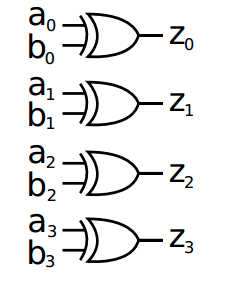
\includegraphics[scale=0.4]{4adder.png}
	\end{center}
	\caption{A 4-bit adder gate level implementation over $\F_2^4$[1]}
	\label{fig:4adder}
\end{figure}

This is a very simple implementation. However, when executing this addition in CPU,
at least a 4-bit addition and a shift operation (for mod $2^4$) will be executed.
Under the same fabrication condition, the hardware implementation cost less time.
\end{Example}

Another advantage can be learnt from above example is the capability of parallel computing.
In this example, each bit during addition is independent from each other. Based on this 
knowledge, the hardware implementation is designed to compute each bit in parallel.
However, a general-purpose CPU must take ordinary sequential computing into consideration
for most bit-dependent additions, so the efficiency of CPU is usually inferior than customized
hardware implementations.

(2) The standard process for CPU to execute an instruction contains some redundant stages.

In example \ref{ex:4adder}, assume this addition is implemented in software. 
If an interpreter is very smart to deduce a 4-parallel-XOR algorithm for this addition 
and the CPU has 4 XOR gates in ALU to execute XOR operation in parallel, can this software 
implementation compete with hardware implementation? The answer is no, because in a combinational
circuit hardware implementation, the input can be read immediately; while in CPU,
there are at least an instruction fetch stage and a decoding stage lagging the whole process.

In conclusion, one advantage of adopting hardware implementations is the higher speed comparing to
software implementations.

\subsection{Other advantages on Hardware implementations}
Besides speed improvement, hardware implementations also have other advantages.
One is less energy consumption. Since there is less time for a customized hardware
design to execute 1 instruction, under the same work load its energy consumption
will be lower than CPU if they work with same power.

In practice, a hardware design may require lower voltage to work, so the power
also could be reduced.

Another advantage is the quality (accuracy) of results. For example, before floating-point unit
(FPU) was embedded into general-purpose CPU, floating-point operations are emulated by CPU 
using a series of simpler fixed-point arithmetic operations that run on integer ALU, the 
accuracy of floating-point computations are limited. Intel 80287 then is an arithmetic hardware
implementation customized for floating-point computations, which is efficient on IEEE 754 compliant
high accuracy floating-point computations. Hardware implementations can be customized to reach 
a higher accuracy which may exceed the CPU limit.

\subsection{Disadvantages on Hardware Implementation}
First disadvantage is loss of convenience. Describing the computation or algorithm in high-level
programming language usually cost relatively short time, while designing layouts and fabrication
cost half to several years in most cases.

Another disadvantage is money cost. A PC/server with general-purpose CPU is standard facility in most labs and 
companies, so there is no extra money cost in software implementations. However, PLDs
and equipments to program PLDs are a fixed expense for hardware implementations. If
the computation is implemented in fully customized design chips, the fabrication charges even
more. I used to send a batch (20 pcs) of 2-inch silicon wafers for simple ion implantations,
the vender charged me more than \$800 for a single process. A set of masks for photolithography
with low resolution ($> 1 \mu m$) pattern costs thousands of dollars. Money is an important 
factor that needs to be taken into consideration.

\subsection{Discussion}
Lots of factors affects the decision to choose hardware implementation or software implementation. 
A balance need to be achieved between disadvantages and advantages while considering their weights
on the decision problem. 

From my point of view, situations to choose hardware implementations includes:\par
(1) Speed/energy consumption/accuracy is greatly improved and they are key factors.
Noticing this point, the FPU was integrated with CPU by Intel and other chip manufacturers.
In labs, when CPU performance is bottleneck in computing, it is also worth
to get a hardware implementation for certain computations/algorithms.\par
(2) If it has to be implemented in hardware. Many computations/algorithms are supposed to be
applied on circuits, such as a secure ID.
 
 \begin{figure}[hbt]
	\begin{center}
	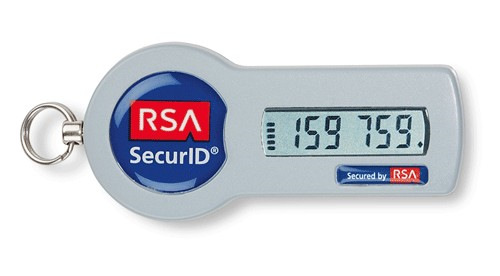
\includegraphics[scale=0.4]{ID.png}
	\end{center}
	\caption{A secure ID based on RSA}
	\label{fig:ID}
\end{figure}
 
\section{Verification of Arithmetic Circuits}
\subsection{Difficulties on Verification}
Control logic is usually implemented through synthesis result of some state graphs.
Each state graph has limited number of states, after state assignment the bit-width
of control signals is relatively small. On the other hand, arithmetic units deal with
numbers (integers, floating-point numbers or polynomials) at word level. Since the computing
logic is not complicated in most case (such as a multiplier), arithmetic unit is easy to
synthesize,i.e. mapping word-level arithmetic function to bit-level boolean functions (gate implementations).
So designer's job is to design an arithmetic unit has the same size required by application.
Unfortunately, the application's request usually covers large-size or high-accuracy input data;
this lead to a wide datapath connecting to arithmetic unit with lots of bits.
\begin{figure}[hbt]
	\begin{center}
	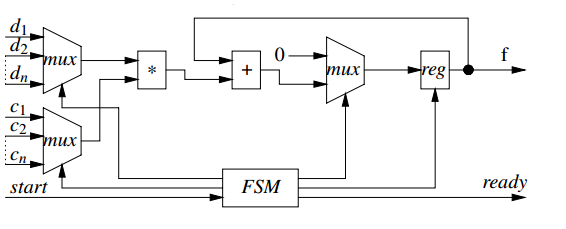
\includegraphics[scale=0.7]{FIR.png}
	\end{center}
	\caption{Comparison between control logic and datapath[2]}
	\label{fig:FIR}
\end{figure}
Fig.\ref{fig:FIR} shows block diagram of order-n FIR filter. It is clear to see there are only
1 bit input and 5 1-bit outputs for the control logic (FSM), but the datapath have 2 $n$-bits
input, $n$ could be a number much larger than 10.

For example, IEEE 754 compliant double precision floating point (round to 0) multiplier has
2 input operands, each of them has 64 bits:

 \begin{figure}[hbt]
	\begin{center}
	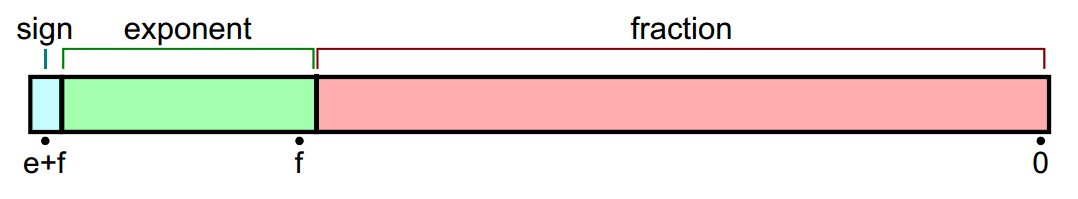
\includegraphics[scale=0.4]{double.png}
	\end{center}
	\caption{Double precision floating-point number in IEEE 754[5]}
	\label{fig:double}
\end{figure}

including 1 sign bit, 11 exponent bits and 52 fraction bits. In total there are 128 bits input,
to exhaustively check all possible inputs, $2^{128}$ test vectors are needed. This is difficult 
to enumerate.

\subsection{Approaches for arithmetic hardware verification}
Verification techniques includes 2 basic types: equivalence checking (EC) and property checking
(PC). Equivalence checking does not suit arithmetic circuit verification very well, because it 
relies on the bit-level miter circuit output, so could not avoid the "bit blasting" issue;
Property checking fits arithmetic verification well because the computational function itself is 
the word-level property need to be checked. To check the property in word-level rather than
bit-level, word-level abstraction techniques are necessary. So in all kind of verification
techniques, those belong to property and can solve the abstraction problem are best techniques
for arithmetic hardware verification.

There are several typical techniques used to address arithmetic circuit verification.
First one is a BDD-like canonical graph-based diagram called Binary Moment Diagram (BMD). [8]
BMDs are used in verifying arithmetic designs with bit-level inputs and integer outputs.
BMDs use modified Shannon's expansion, where Boolean variable is treated as binary integer 
variable. For example, the complement of variable $x$ is modeled as $\bar{x} = 1-x$
and according to Shannon's expansion
$$f(x) = (1-x)\cdot f_{\bar{x}} + x\cdot f_x = f_{\bar{x}} + x\cdot(f_x - f_{\bar{x}}) = f_{\bar{x}} + x\cdot f_{\Delta x}$$
The above decomposition is called \emph{moment} decomposition where $f_{\bar{x}}$ is the 
\emph{constant moment}, $f_{\Delta x}$ is the \emph{linear moment}. In this way a Boolean
function $f$ is "transformed" to a linear function of $x$.
 \begin{figure}[hbt]
	\begin{center}
	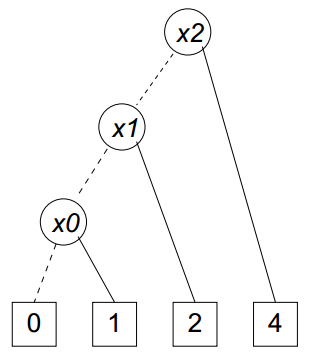
\includegraphics[scale=0.4]{BMD.png}
	\end{center}
	\caption{An example of BMD[8]}
	\label{fig:BMD}
\end{figure}
Fig.\ref{fig:BMD} is an example of BMD representation, it stands for an integer encoded
by 3 bits: $X = 4x_2 + 2x_1 + x_0$,
dashed edges means the constant moment and solid edges represent the first moment of the function 
w.r.t. the decomposing variable. As an application, a word-level BMD can efficiently represent an integer multiplication
because its size grows linearly with the size of multiplier's input, which is easy to observe
from fig.\ref{fig:multi} 
 \begin{figure}[hbt]
	\begin{center}
	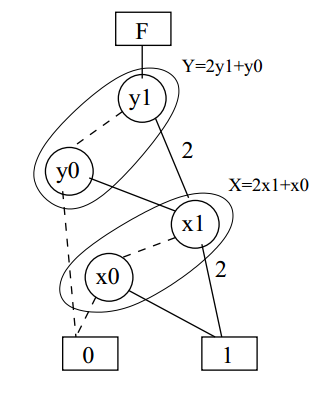
\includegraphics[scale=0.4]{multi.png}
	\end{center}
	\caption{BMD for $F = x \cdot y$, $x,y$ are 2-bit words, $F$ is 4-bit word[1]}
	\label{fig:multi}
\end{figure}

Another approach is \emph{Tylor Expansion Diagram} (TED)[1]. The abstraction method of TED is borrowed
from Tylor series expansion. Assume a Boolean function $f(x,y,\dots)$ be differentiable, it can 
be expanded w.r.t. variable $x$:
$$f(x,y,\dots) = f(x=0,y,\dots) + x\cdot f'(x=0,y,\dots) + \frac{1}{2}x^2\cdot f''(x=0,y,\dots) + \cdots$$
and it can be further expanded on remaining variables because taking $x=0$ already ensure any derivatives of $f$ are 
independent from $x$; recursive decomposition results a tree which is $TED$.

Moreover, some symbolic algebraic methods also provide effective abstraction. Dr. Kalla [3] proposed
an abstraction based on computing the Gr\"obner basis with abstraction term order on 
elimination ideal, the approach will directly given out the polynomial of system specification,
which can be compared to equations from arithmetic computations.

\subsection{Discussion}
Although I mentioned several approaches suit arithmetic verification well, till now there is 
no optimal method can deal with all arithmetic verification problems. There are many limitations
on the applications of those approaches.

One of the main limitations of BMD is that performing certain arithmetic operations cost badly,
such as power function and modular operations; TED has similar limitations as BMD. For Gr\"obner
basis approach, modeling method on complex arithmetic designs for integers has not been developed,
and in general case Gr\"obner basis computing costs exponential complexity time, symbolic algebraic 
tools have not yet been widely used.

In conclusion, the nature of difficulties is lack of computing capabilities so that it is 
not practical to exhaust $O(2^n)$ input search space. In order to get around this problem,
some approaches are proposed but they can only be effective/efficient to part of original 
problems.

\section{Prevention from design flaws}
\subsection{Intel FDIV bug}
The Intel FDIV bug occurs in 5 entries in the lookup table (LUT) of SRT division for floating-point
division algorithm in Pentium processor.

{\bf SRT Division} is a fast division algorithm widely adopted in CPU/FPU computing.
It is highly similar to the long division method we learned from elementary school,
the only difference is:
given dividend $p_0$ and divisor $d$, within each iteration $i$, $p_i$ is temporary 
dividend, the partial quotient
$q_i$ is chosen to satisfy
$$0\leq p_i - q_i\cdot d < d \ \ \ \ (\text{for long division})$$
$$|p_i - q_i\cdot d| \leq \frac{k}{r}\cdot d\ \ \ \ (\text{for $r$-radix SRT division})$$

Radix $r$ limits the range of quotient we can choose from, $k$ is a parameter
calculated according to $r$ to guarantee at every iteration only reasonable value of partial quotient
falls into interval $[-\frac{k}{r}\cdot d, \frac{k}{r}\cdot d]$.

\begin{Example}
Assume $r=10$, which means partial quotient could take value from $\{-5,-4,\dots,4,5\}$
corresponding $k/r = 5/9$.

Given dividend $p_0 = 1.000$, divisor $d = 8.000$, now compute 1/8.

Iteration 1: Choose first digit of quotient $q_0$ so that $|p_0-q_0\cdot d|\leq \frac{5}{9}\cdot 8.000$.
The only candidate is $q_0 = 0$. Then compute temporary dividend for next iteration:
\[
p_1 = 10\cdot(1.000 - 0\cdot 8.000) = 10.000
\]

Iteration 2: Choose $q_1$ so that $|10.000-q_1\cdot 8.000|\leq \frac{5}{9}\cdot 8.000$.
The only choice is $q_1 = 1$.
$$p_2 = 10\cdot(10.000 - 1\cdot 8.000) = 20.000$$

Iteration 3: Choose $q_2$ so that $|20.000-q_2\cdot 8.000|\leq \frac{5}{9}\cdot 8.000$.
Now there are two candidates, 2 and 3. Assume the algorithm chooses $q_2 = 3$ (can be either
deterministically or nondeterministically).
$$p_3 = 10\cdot(20.000 - 3\cdot 8.000) = -40.000$$

Iteration 4: Choose $q_3$ so that $|-40.000-q_3\cdot 8.000|\leq \frac{5}{9}\cdot 8.000$.
$q_3 = -5$ is the only choice.
$$p_4 = 10\cdot(-40.000 - (-5\cdot 8.000)) = 0.000$$
Algorithm terminates. The final quotient is $0+0.1+0.03+(-0.005) = 0.125$. [6]
\end{Example}

The SRT division adopted by FDIV has $r = 4$, which means quotient can be chosen
from $\{-2,-1,0,1,2\}$, and corresponding $k/r = 2/3$. If temporary dividend is given,
then the possible value(s) of quotient can be computed. In order to achieve higher efficiency,
FDIV uses LUT shown on last page (source: http://daviddeley.com/pentbug/pentbug3.htm).
As soon as FDIV algorithm get temporary dividend $p_i$, in LUT, unit $(d,p_i)$ stores
the value of corresponding quotient, reading from LUT cost $O(1)$ time.

This LUT is implemented in forms of PLA.[10] The bug occurs at 5 red units (also shown on last page),
in these units, pre-stored quotient value should be 2, but they are all equal to 0 in the buggy FPU.[4]
These 5 units are rarely used in most divisions, so the bug failed to be detected by test engineer
from Intel.

\subsection{Detection of similar flaws}
This LUT passed Intel's validation, because the prover only checked the lower half of
LUT (which is correct) and believed the upper half would be mirror to lower half.
After chips were fabricated, Intel also test it with millions of test vectors, unfortunately
no one hit this bug. This indicates that a formal method which can cover all possible
input logic is necessary.

I have 2 suggestions to detect this kind of bugs. One is to verify the synthesis result 
(values assigned to LUT) with a theorem prover such as HOL and PVS. In this example, for 
each $unit(d,p_i)$, check whether assertion 
$$|p_i - unit(d,p_i)\cdot d| \leq \frac{2}{3}\cdot d$$
is satisfied. Similar checking can be embedded into the synthesis tool, to eliminate bugs
inside synthesis tools (software verification).

The other one is to build a built-in module for test. This module could be designed based on 
the property we are aiming. For example, if we build an adder module to calculate 
the sum of all entries in LUT, a lot of bugs can be detected (including this FDIV bug)
except which does not change the sum. By designing reasonable built-in test modules,
time for test could be shorter while the coverage on bugs will be improved.

\subsection{Discussion}
The first paper[7] uses a lot of implementations in HOL theorem prover to argue that any theorems
adopted by floating-point algorithm synthesis tools can be verified. One of these implementations
is:

The following theorem can be implemented with HOL theorem prover statements in fig.\ref{fig:HOL}:
\begin{Theorem}
\label{alg:HOL}
If $q$ is a floating point number within 1 $ulp$ of the true quotient $a/b$ of two floating point
numbers, and $y$ is the correctly rounded-to-nearest approximation of the exact reciprocal $\frac{1}{b}$,
then the following two floating point operations:
$$r = a - bq$$
$$q' = q+ry$$
using round-to-nearest in each case, yield the correctly round-to-nearest quotient $q'$.
 \begin{figure}[hbt]
	\begin{center}
	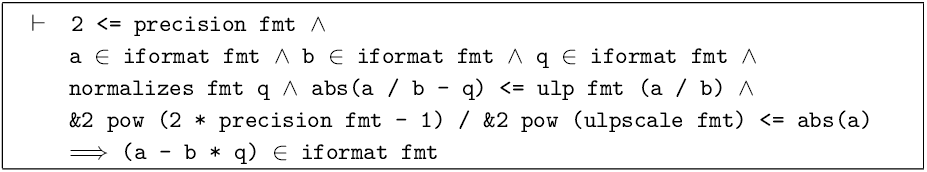
\includegraphics[scale=0.6]{HOL.png}
	\end{center}
	\caption{HOL statements to prove theorem \ref{alg:HOL}[7]}
	\label{fig:HOL}
\end{figure}
\end{Theorem}

There is a whole argument on applying HOL prover to verify Intel Itanium floating point architecture,
which supports my suggestion on using theorem provers.

The second paper[9] talks about the built-in self speed test (BISST). BISST supports my ideal about
built-in test module, but works in slightly different way. Fig.\ref{fig:BISST} describes the implementation 
of BISST. First, only key function modules are tested; second, the essential idea of BISST is to 
build a bug-free module realizing the same function, then use a miter structure to check equivalence
of outputs; third, the BISST can be activated separately when testing.

\begin{figure}[hbt]
	\begin{center}
	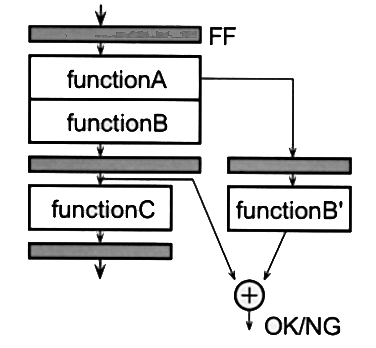
\includegraphics[scale=0.4]{BISST.png}
	\end{center}
	\caption{A block diagram for BISST[9]}
	\label{fig:BISST}
\end{figure}

This paper also talked about an issue which my suggestion does not concern. To build a 
bug-free copy for every key module will occupy too much area, so this paper discussed how to
shrink the output signals so that the area cost could be lower down and keep a reasonable probability
of aliasing. In my suggestion, every module is designed as a property checker, so it will have much
smaller size than the module it tests. 

%%%%%%%%%%%%%%%%%%%% The bibliography %%%%%%%%%%%%%%%%%%%%%%%%%%%%
\begin{thebibliography}{1}

\bibitem{ref1}
Lv, Jinpeng. Scalable formal Verification of finite field Arithmetic circuits using
computer algebra techniques. Diss. University of Utah, 
Dept. of Electrical and Computer Engineering, 2012.

\bibitem{ref2}
Raudvere, Tarvo, et al. "System level verification of digital signal processing applications based on the polynomial abstraction technique." Computer-Aided Design, 2005. ICCAD-2005. IEEE/ACM International Conference on. IEEE, 2005.

\bibitem{ref3}
T. Pruss, P. Kalla and F. Enescu. Word-level Abstraction from Bit-level circuits using Gr\"obner Bases. IWLS 2013



\bibitem{ref4}
David W. Deley. "The Pentium Divison Flaw". 

\bibitem{ref5}

Wikipedia: IEEE 754. http://en.wikipedia.org/wiki/IEEE\_floating\_point

\bibitem{ref6}

Clarke, Edmund M., Steven M. German, and Xudong Zhao. "Verifying the SRT division algorithm using theorem proving techniques." Computer Aided Verification. Springer Berlin Heidelberg, 1996.
\bibitem{ref7}

Harrison J. \emph{Floating-point verification using theorem proving[M]. Formal Methods for Hardware Verification}. Springer Berlin Heidelberg, 2006: 211-242.

\bibitem{ref8}

Chen Y A. \emph{Arithmetic circuit verification based on word-level decision diagrams}[D]. Intel, 1998.

\bibitem{ref9}

Hagihara, Yasuhiko, et al. "Floating-point datapaths with online built-in self speed test." Solid-State Circuits, IEEE Journal of 32.3 (1997): 444-449.

\bibitem{ref10}

Price D. \emph{Pentium FDIV flaw-lessons learned}[J]. Micro, IEEE, 1995, 15(2): 86-88.

\end{thebibliography}

\end{document}

%%%%%%%%%%%%%%%%%%%%%%%%%%%  End of IEEEsample.tex  %%%%%%%%%%%%%%%%%%%%%%%%%%%